\subsection{Abbildungen}						% aufgabe 6
\pagecolor{white}
\begin{aufgabe}\label{aufg:fig} \label{aufg:22}
F\"ugen Sie ein beliebiges Bild ein, das 10\,cm breit ist und oben und unten um 1cm zurecht geschnitten wurde. 
\end{aufgabe}

\afterpage{
\begin{figure}[t] 								% aufgabe 25
\centering 									% aufgabe 25
\setlength{\fboxrule}{1pt} 							% aufgabe 24
% aufgabe 21
\fbox{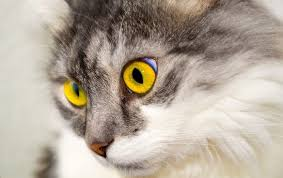
\includegraphics[width=10cm,clip=true,trim= 0cm 1cm 0cm 1cm]{cat.jpg}} 	% aufgabe 22
\caption[Die Katzen (Felidae)]
	{Dies ist eine süße kleine Katze im Miniformat. Aaaaawww\dots\\
	\glqq Die Katzen (Felidae) sind eine Familie aus der Ordnung der Raubtiere (Carnivora) innerhalb der Überfamilie
	der Katzenartigen (Feloidea). Sie sind auf allen Kontinenten außer Ozeanien und Antarktika verbreitet und 
	nahezu ausschließlich Fleischfresser. Eingeteilt werden sie in Großkatzen (wie beispielsweise Löwe, Tiger 
	und Leopard) und Kleinkatzen (etwa Wildkatze, Luchs und Ozelot), wobei zu den Kleinkatzen auch große
	Vertreter wie der Puma und – nach neueren molekulargenetischen Erkenntnissen – der Gepard gehören. 
	Mit der von der Wildkatze abstammenden Hauskatze wurde ein Vertreter der Familie durch Domestizierung 
	zu einem Begleiter des Menschen.\grqq \\ (aus https://de.wikipedia.org/wiki/Katzen, 23.08.2017)}	
\label{abb:cat} 		% aufgabe 24
\end{figure}}

\begin{aufgabe}
\label{aufg:23}
Legen Sie das Bild aus der vorherigen Aufgabe in ein eigenes Verzeichnis f\"ur Abbildungen. \"Ubergeben Sie \LaTeX\ das Abbildungsverzeichnis global.	
\end{aufgabe}

\begin{aufgabe}
\label{aufg:24}
Rahmen Sie die Abbildung aus Aufgabe~\ref{aufg:fig} mit einem 1\,pt dicken Rahmen ein.
\end{aufgabe}

\begin{aufgabe}
\label{aufg:25}
Setzen Sie die Abbildung aus Aufgabe~\ref{aufg:fig} in eine Float Umgebung und f\"ugen Sie ihr eine geeignete Bildunterschrift hinzu, welche \"uber mehrere Zeilen reicht. Die Abbildung soll sich am oberen Seitenrand befinden und zentriert sein. Schreiben Sie unter diese Aufgabe einen Satz, in dem Sie auf die Abbildung verweisen.	
\end{aufgabe}
\FloatBarrier			% aufgabe 30
In der Bildunterschrift der Abbildung \ref{abb:cat} wird der Einleitungstext aus dem Wikipedia-Artikel über Katzen zitiert.

\pagebreak
\begin{aufgabe}
F\"ugen Sie eine weitere Abbildung in einer weiteren  Float Umgebung ein. 
Die Abbildung soll 14\,cm hoch sein, aber nicht \"uber den Seitenrand hinaus gehen. 
Die Abbildung soll eine geeignete mehrzeilige Bildunterschrift erhalten. 
Die Abbildung soll sich \textsc{nicht} auf einer einzelnen Seite befinden.
\end{aufgabe}

\FloatBarrier
\begin{figure}[h]
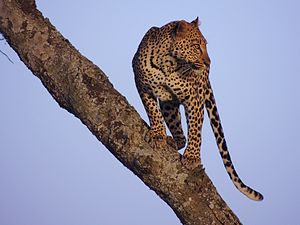
\includegraphics[height=14cm, width=\textwidth, keepaspectratio=false]{leo}
\caption[Der Leopard (Panthera pardus)]
	{Der Leopard (Panthera pardus) ist eine Art aus der Familie der Katzen, die in Afrika und Asien verbreitet ist.}
\end{figure}
\FloatBarrier


\begin{aufgabe}
F\"ugen Sie dem Protokoll ein Abbildungsverzeichnis hinzu. Die Bildunterschriften im Abbildungsverzeichnis sollen nicht \"uber eine Zeile hinaus gehen.
\end{aufgabe}

\pagebreak
\begin{aufgabe}
F\"ugen Sie zwei Abbildungen (Bannerformat) untereinander ein. 
Die Abbildungen sollen jeweils eine eigene und eine gemeinsame Bildunterschrift erhalten. 
Verweisen sie auf eine der beiden Teilabbildungen.

\begin{figure}[h]
 \begin{subfigure}[h]{\textwidth}
  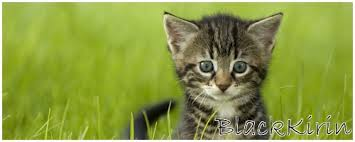
\includegraphics[width=\textwidth]{ban1.jpg}
  \caption{Das ist die erste Banner Katze.}
  \label{abb:banner1}
 \end{subfigure}
 
 \begin{subfigure}[h]{\textwidth}
  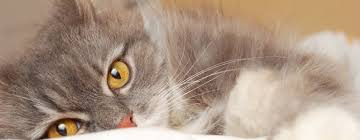
\includegraphics[width=\textwidth]{ban2.jpg}
    \caption{Das ist die zweite Banner Katze.}
 \end{subfigure}
  
 \caption{Diese Abbildung verdeutlicht den Vorteil von Subfigure~-~Umgebungen.}
\end{figure}
\end{aufgabe}
\FloatBarrier
Besonders katzig ist die Bannerkatze aus Abbildung \ref{abb:banner1}.

\pagebreak
\begin{aufgabe}
F\"ugen Sie zwei Abbildungen nebeneinander ein. Die Abbildungen sollen die gleiche H\"ohe haben und jeweils eine eigene und eine gemeinsame Bildunterschrift erhalten.

\begin{figure}
 \centering
 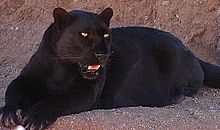
\includegraphics[height=3cm]{blacky}
 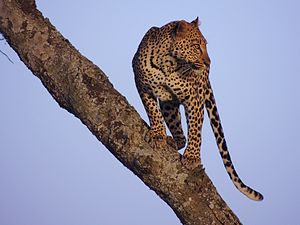
\includegraphics[height=3cm]{leo}
\caption{Diese beiden Tiere gehören derselben Art Katze an.}
\label{img:nebeneinander}
\end{figure}
\end{aufgabe}
\noindent (Abbildung \ref{img:nebeneinander} oberhalb der Aufgabenstellung.)


\begin{aufgabe}
Verwenden Sie einen geeigneten Befehl, damit keine der Abbildungen nach der n\"achsten Aufgabe erscheint.
\end{aufgabe}
Da die Aufgaben \ref{aufg:22}, \ref{aufg:23}, \ref{aufg:24}, \ref{aufg:25} sich alle auf ein Bild (Abbildung \ref{abb:cat}) beziehen,
habe ich dieses Bild auf die nächste Seite gelegt.
Dadurch wird auch das Design nicht zerstückelt.
Ich wollte, dass die Kapitelüberschrift von Kapitel \ref{sec:floats} auf einer neuen Seite (Seite \pageref{abb:cat}) steht.
Wäre zuerst das Bild gekommen, wäre das uneinheitlich gegenüber dem Gesamtaussehen des Protokolls gewesen.

\pagebreak
\subsection{Tabellen}							% aufgabe 6
\begin{aufgabe}
\TeX en Sie folgende Tabelle so exakt wie m\"oglich nach.	
\end{aufgabe}

\noindent \underline{Ursprung:} \\
\noindent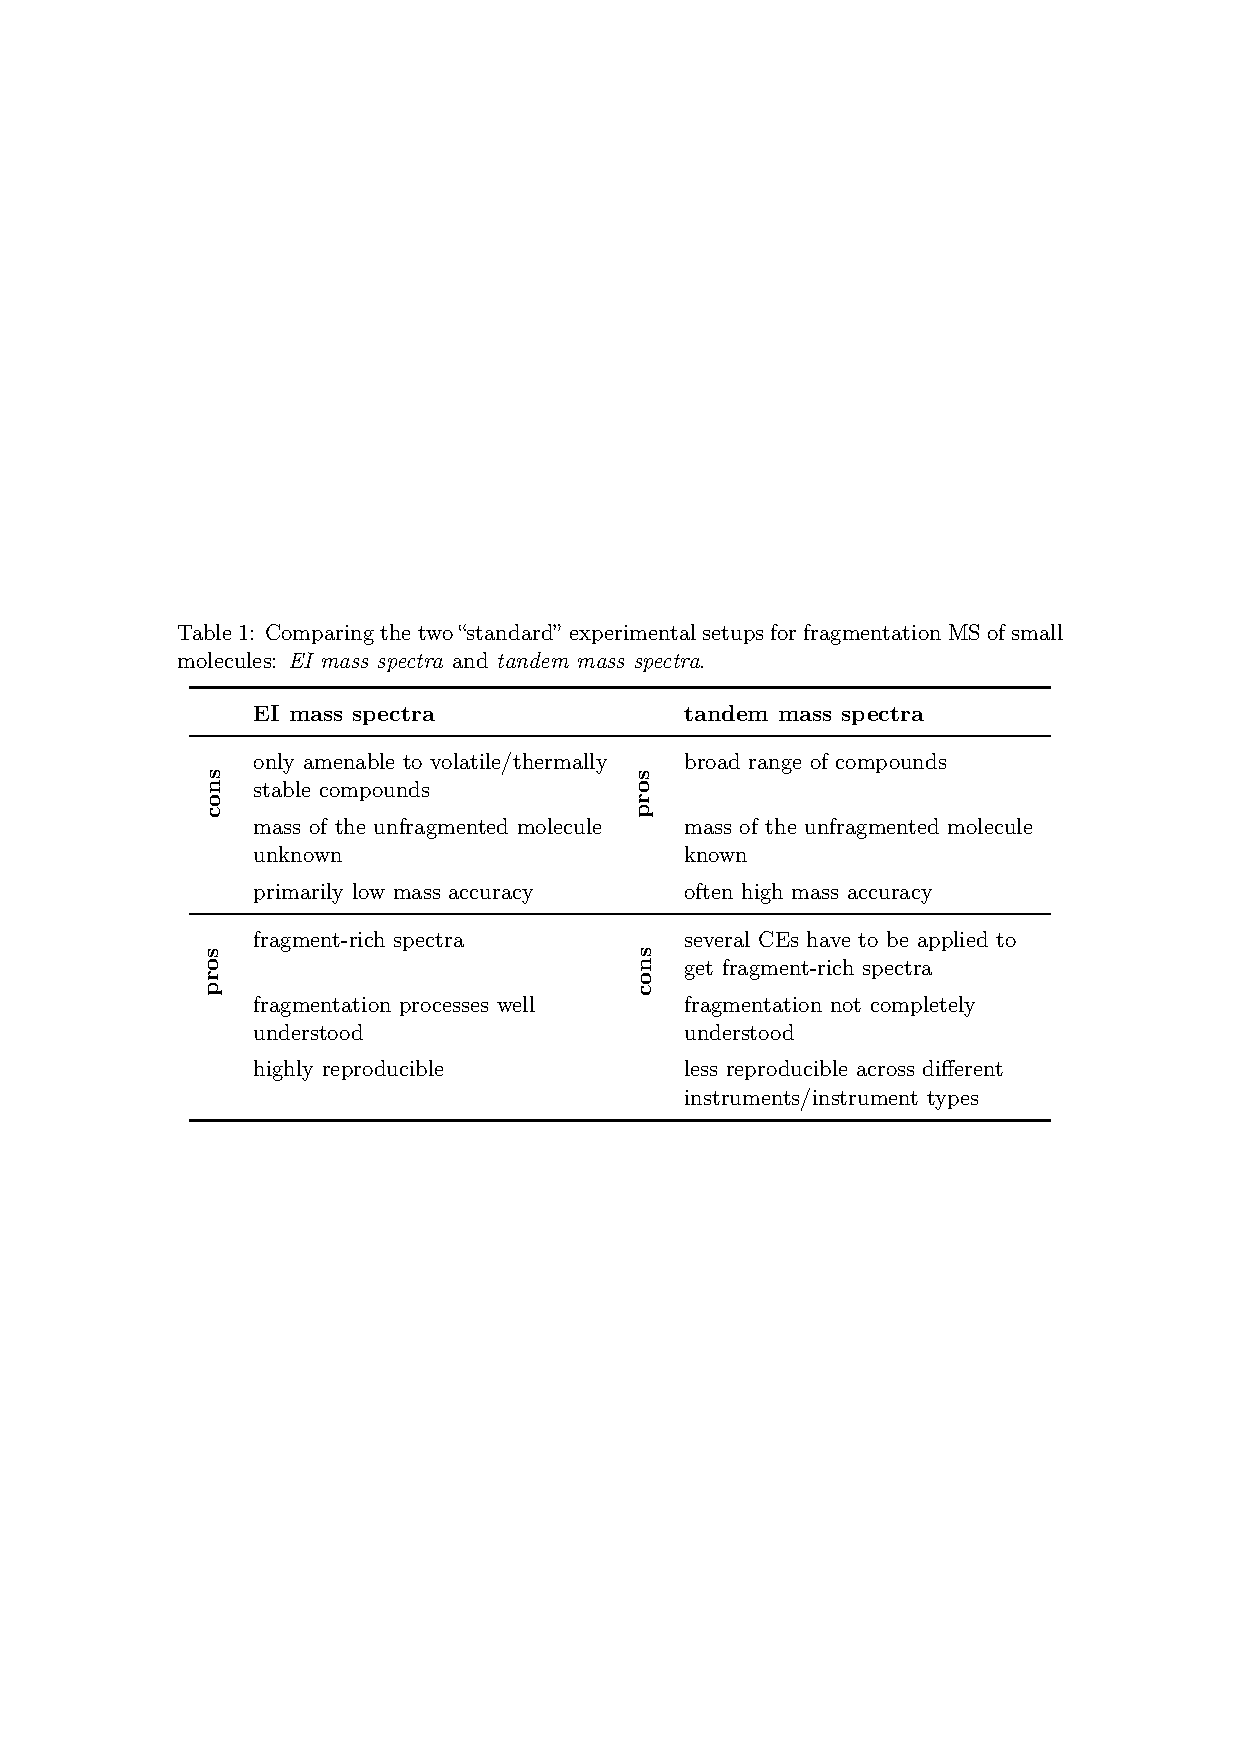
\includegraphics[width=\textwidth]{aufgabe31}

\noindent \underline{nachge\TeX t:}\\
\FloatBarrier
\begin{table}[H]
\selectlanguage{english}
 \caption[Comparing the two “standard” experimental setups for fragmentation MS]
	 {Comparing the two “standard” experimental setups for fragmentation MS of small
	  molecules: \textit{EI mass spectra} and \textit{tandem mass spectra}.\\
	  }
	  \vspace{-0.6cm} \hspace{2mm}
\begin{tabularx}{\textwidth}{p{0.04\textwidth} p{0.4\textwidth} p{0.04\textwidth} p{0.4\textwidth}}
 \toprule
 & \textbf{EI mass spectra} &  & \textbf{tandem mass spectra} \\
 \midrule
    \multirow{3}*{\begin{sideways} \textbf{cons} \end{sideways}}
  & only amenable to volatile/thermally
    stable compounds\newline
    mass of the unfragmented molecule
    unknown\newline
    primarily low mass accuracy\newline
  & \multirow{3}*{\begin{sideways} \textbf{pros} \end{sideways}}  
  & broad range of compounds\newline \newline
    mass of the unfragmented molecule
    known\newline
    often high mass accuracy\\
    \midrule
    \multirow{3}*{\begin{sideways} \textbf{pros} \end{sideways}}
  & fragment-rich spectra\newline
    \newline
    \raggedright{ processes well
    understood}\newline
    highly reproducible
  & \multirow{3}*{\begin{sideways} \textbf{cons} \end{sideways}}
  & several CEs have to be applied to
    get fragment-rich spectra\newline
    fragmentation not completely
    understood\newline
    less reproducible across different
    instruments/instrument types\\
 \bottomrule
\end{tabularx}
\end{table}

\pagebreak
\begin{aufgabe}
\TeX en Sie folgende Tabelle so exakt wie m\"oglich nach.		
\end{aufgabe}
\FloatBarrier
\noindent \underline{Ursprung:} \\
\noindent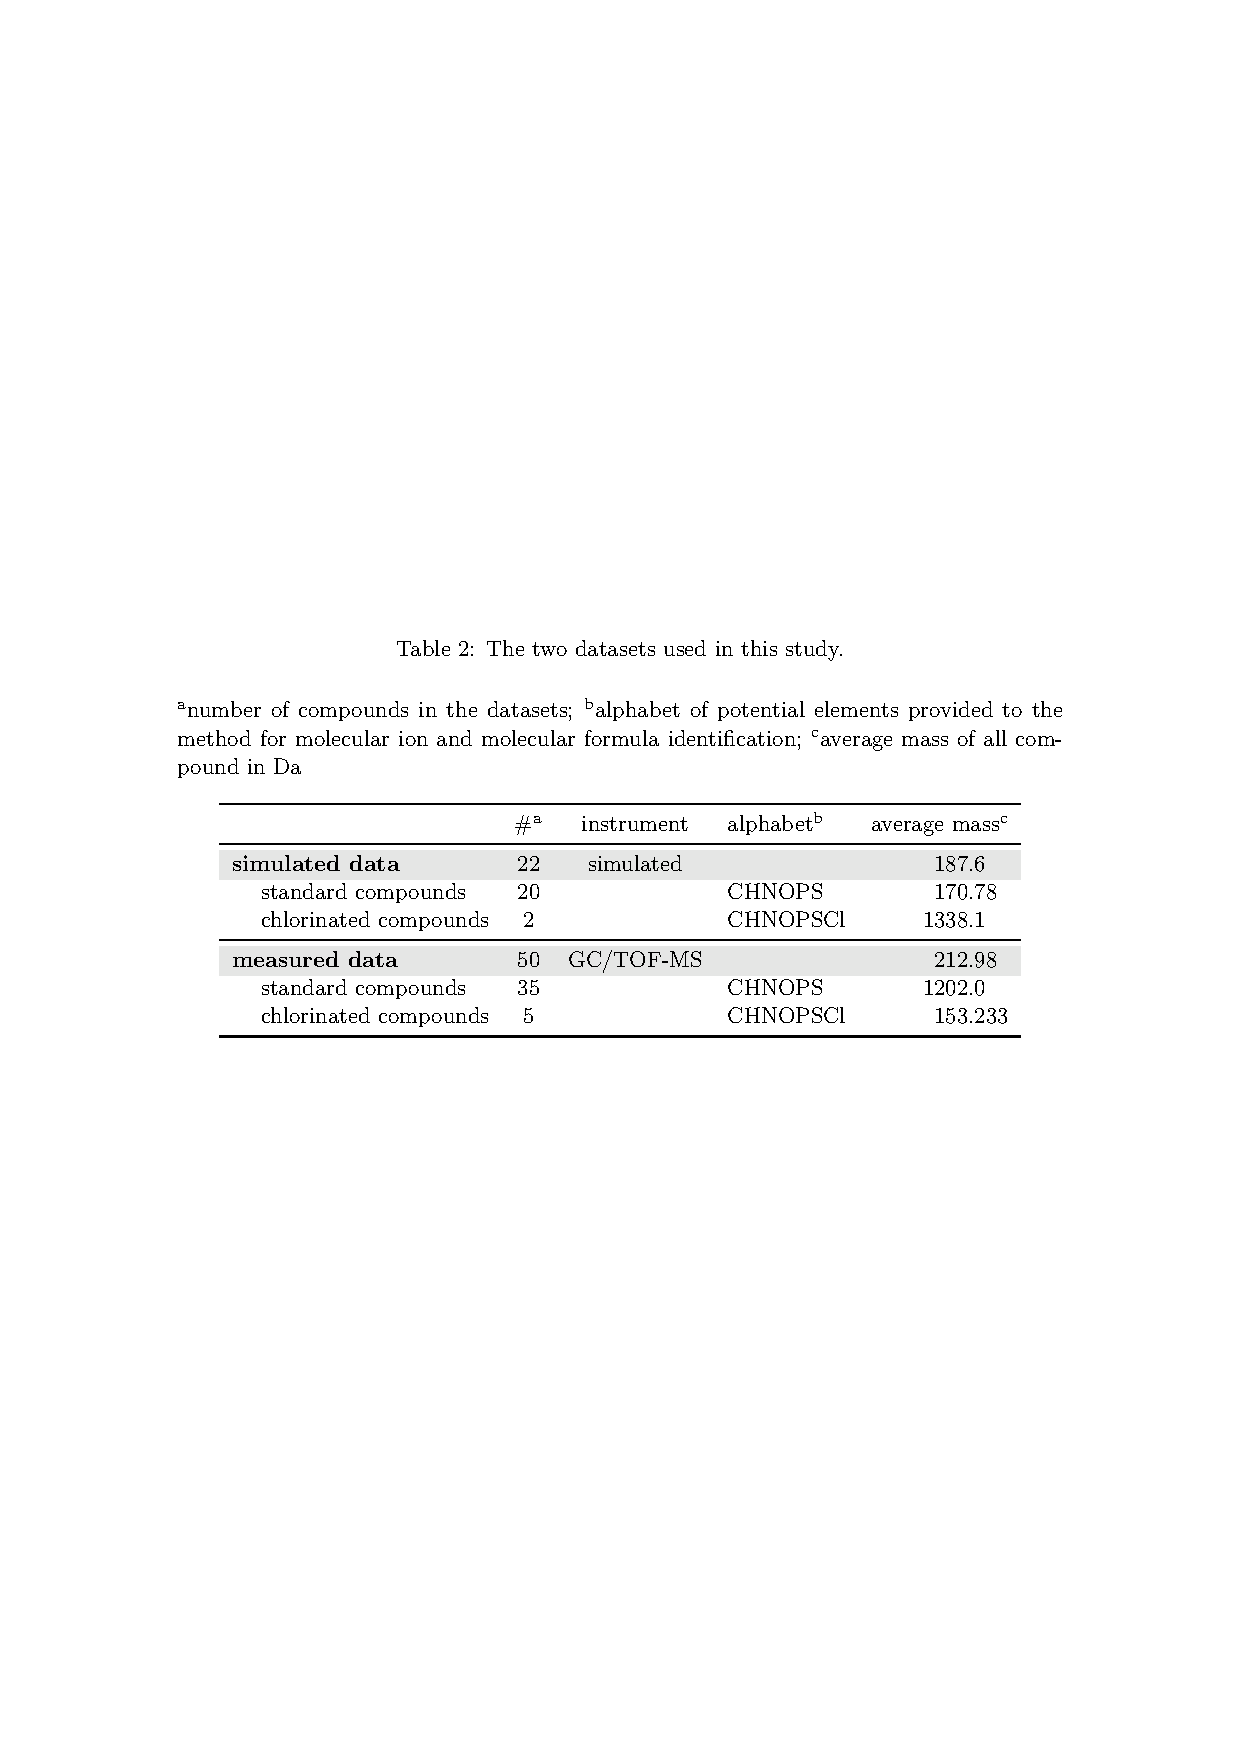
\includegraphics[width=\textwidth]{aufgabe32}
\\
\noindent \underline{nachge\TeX t:}\\
\indent
\begin{table}
\selectlanguage{english}
\caption{The two datasets used in this study.}
\caption*{
\textsuperscript{a}\hspace{-1mm} number of compounds in the datasets; 
\textsuperscript{b}\hspace{-1mm} alphabet of potential elements provided 
				 to the method for molecular ion and molecular formula identification; 
\textsuperscript{c}\hspace{-1mm} average mass of all com- \-pound in Da 
}
\hspace*{0.48cm}
\begin{tabularx}{0.91\textwidth}{llcle{2}}
 \toprule 
				       & \#\textsuperscript{a} 
				       & instrument 
				       & alphabet\textsuperscript{b} 
				       & \textrm{average mass}\textsuperscript{c}\\
 \midrule
 \rowcolor{LessLightGrey}
 \textbf{simulated data} 	       & 22	    & simulated  &              &  187.6\\
 \hspace{0.41cm} standard compounds    & 20	    & 		 & CHNOPS	& 170.78\\
 \hspace{0.41cm} chlorinated compounds & 35	    &            & CHNOPSCl     & 1338.1\\
 \midrule
 \rowcolor{LessLightGrey}
 \textbf{measured data}	       	       & 50         & GC/TOF-MS  & 		& 212.98\\
 \hspace{0.41cm} standard compounds    & 35         & 		 & CHNOPS	& 1202.0\\
 \hspace{0.41cm} chlorinated compounds & 5	    &            & CHNOPSCl     & 153.233\\
 \bottomrule 
  \end{tabularx}
\end{table}

\pagebreak
\begin{aufgabe}
F\"ugen Sie dem Dokument ein Tabellenverzeichnis hinzu. Abbildungs- und Tabellenverzeichnis sollen gemeinsam auf einer eigenen Seite stehen. Die Tabellenunterschriften im Tabellenverzeichnis sollen nicht \"uber eine Zeile hinaus gehen.	
\end{aufgabe}
